\section{Supplement}

This section contains algorithms, proofs, and experiments in support of the main text.

\subsection{Algorithms}
\label{sec:algorithms}

We give definitions of the brute and greedy algorithms for the combinatorial problem studied in this paper.
The brute force algorithm is computationally intractable for all but the smallest problems, but always finds the global minima.

\begin{algorithm}[H]
\caption{\brute(Matrix ${X} \in \mathbb{R}^{D \times P}$, objective $f$)}
\begin{algorithmic}[1]
\FOR{each combination $S \subseteq \{1, 2, \dots, P\}$ with $|S| = D$}
    \STATE Evaluate $f({X}_{.S})$
\ENDFOR
\STATE {\bf Output} the combination $S^*$ that minimizes $f({X}_{.S})$
\end{algorithmic}
\end{algorithm}

Greedy algorithms are computationally expedient but can get stuck in local optima \citep{Cormen, Russell-09}, even with randomized restarts \citep{Dick2014HowMR}.

\begin{algorithm}[H]
\caption{\greedy(Matrix ${X} \in \mathbb{R}^{D \times P}$, objective $f$, selected set $S = \emptyset$, current size $d=0$)}
\begin{algorithmic}[1]
\IF{$d = D$}
    \STATE {\bf Return} $S$
\ELSE
    \STATE {\bf Initialize} $S_{\text{best}} = S$
    \STATE {\bf Initialize} $f_{\text{best}} = \infty$
    \FOR{each $p \in \{1, 2, \dots, P\} \setminus S$}
        \STATE {\bf Evaluate} $f({X}_{.(S \cup \{p\})})$
        \IF{$f({X}_{.(S \cup \{p\})}) < f_{\text{best}}$}
            \STATE {\bf Update} $S_{\text{best}} = S \cup \{p\}$
            \STATE {\bf Update} $f_{\text{best}} = f(\mathcal{X}_{.(S \cup \{p\})})$
        \ENDIF
    \ENDFOR
    \STATE {\bf Return} \greedy(${X}$, $f$, $S_{\text{best}}$, $d+1$)
\ENDIF
\end{algorithmic}
\end{algorithm}

\subsection{Proofs}
\label{sec:proofs}

\subsubsection{Proof of Proposition \ref{prop:basis_pursuit_selection_invariance}}
\label{proof:basis_pursuit_program_invariance}

In this proof we first show that the penalty $\|\beta\|_{1,2}$ is unchanged by unitary transformation of $\beta$.

 \begin{proposition}
 \label{prop:basis_pursuit_loss_equivalence}
 Let $U \in \mathbb R^{D \times D}$ be unitary.
 Then $\|\beta\|_{1,2} = \|\beta U \|$.
\end{proposition}

\begin{proof}
\begin{align}
\|\beta U \|_{1,2} &= \sum_{p = 1}^P \| \beta_{p.} U \| \\
&= \sum_{p = 1}^P \| \beta_{p.} \| \\
&= \|\beta \|_{1,2}
\end{align}
\end{proof}

We then show that this implies that the resultant loss is unchanged by unitary transformation of $ X$.

\begin{proposition}
 \label{prop:basis_pursuit_loss_equivalence}
 Let $U \in \mathbb R^{D \times D}$ be unitary.
 Then $\widehat \beta  (U  X) = \widehat \beta  (  X) U$.
\end{proposition}

\begin{proof}
\begin{align}
\widehat \beta  (U  X)  &= \arg \min_{\beta \in \mathbb R^{P \times D}} \|\beta\|_{1,2}  \; : \; I_{D} = U X \beta \\
&= \arg \min_{\beta \in \mathbb R^{P \times D}} \|\beta\|_{1,2}  \; : \; U^{-1} U = U^{-1} U X \beta U \\
&= \arg \min_{\beta \in \mathbb R^{P \times D}} \|\beta\|_{1,2}  \; : \;  I_D = X \beta U \\
&= \arg \min_{\beta \in \mathbb R^{P \times D}} \|\beta U \|_{1,2}  \; : \;  I_D = X \beta U \\
&= \arg \min_{\beta \in \mathbb R^{P \times D}} \|\beta \|_{1,2}  \; : \;  I_D = X \beta.
\end{align}
\end{proof}

\subsubsection{Proof of Proposition \ref{prop:unitary_selection}}
\label{proof:unitary_selection}

In this proof we first show that the orthonormal submatrix $X_{.S}$ is contained within the set $\widehat \mathcal \beta_{MBP} (w(X,c), I_D)$.

\begin{proposition}
\label{prop:kkt}
Let $X_{.S}$ be a rank $D$ orthonormal submatrix of $X$.
Then $S \in S(\beta) : \beta \in \widehat \mathcal \beta_{MBP} (w(X,c), I_D))$.
 \end{proposition}
 
 \begin{proof}
 
 By Proposition \ref{prop:basis_pursuit_selection_invariance} without loss of generality, let $X_{.S} = I_D$.
 Also, without loss of generality let $S = \{1 \dotsc D\}$.
 We show that $\beta = [I_D 0]$ satisfies the KKT conditions for $X = [I_D X_{-S}]$.
 
Recall that the KKT conditions for a convex optimization problem are a set of conditions on an element of the domain of the optimization algorithm that, if satisfied, certify that the element is a solution.
To write out the KKT conditions, we define the Lagrangian
\begin{align}
\mathcal L(X,\beta,\nu) = \|\beta\|_{1,2} + \nu^T (I_D - w(X,c) \beta)
\end{align}
where $\nu \in \mathbb R^{D\times D}$ is the dual variable.

The KKT conditions are then
\begin{itemize}
\item Primal feasibility: $w(X, c) \beta = I_D$
\item Stationarity: there exists a dual variable $\nu$ such that $0 \in \partial \|\beta\|_{1,2} - w(X, c)^T \nu$  where $\partial$ is the subdifferential operator.
\end{itemize}
where dual feasibility and complementary slackness are ignorable by virtue of the absence of inequality constraints.

First note that in our case, primal feasibility is satisfied by $X$ being rank $D$ and $w$ not effecting the rank of the transformed matrix since it only rescales length and not direction.

For stationarity, recall that 
\begin{align}
\|\beta\|_{1,2} = \sum_{p = 1}^P \|\beta_{p.}\|_2.
\end{align}
Then, by the definition of subdifferential
\begin{align}
\partial \|\beta\|_{1,2} = \begin{bmatrix}
I_D
v_{d+1} \\
\dotsc \\
v_P
\end{bmatrix}
\end{align}
where $v_p \in \mathbb R^{D}$ can be any vector satisfying $\|v_p\|_2 \leq 1$.

We therefore must show that there exists a $\nu$ that satisfies
\begin{align}
\begin{bmatrix}
I_D \\
w(X_{-S},c)^T
\end{bmatrix}\nu  = \begin{bmatrix}
I_D \\
V_{-S}
\end{bmatrix}.
\end{align}
At this point we can see that in fact $I_D$ is an appropriate choice of $\nu$ since normalization by $w$ leads to vectors satisfying $\|w(X,c\|_2 \leq 1$.

Since for this $\beta$, $S(\beta) = S$, we have shown that $S$ is the support of a solution to $\beta_{MBP} (w(X,c), I_D)$.
\end{proof}

The next part of the proof handles the presence of non-unique solutions.

\begin{proposition}
\label{prop:support_containment}
$S(\widehat \beta_c ( X)) = \cup S(\beta): \beta \in  \mathcal \beta_{MBP} (w(X,c), I_D)$
 \end{proposition}

\begin{proof}
The proposition follows from geometric properties of the solution set.
We ignore the case for singleton solutions, for which the proposition is obvious.
Recall that $\widehat \beta_c ( X) := \widehat \beta_{MBP}^{\ell_2} ( w(X,c), I_D ) =  \arg \min_{\beta \in \mathbb R^{P \times D} } \|\beta\|_F : \beta \in \widehat \mathcal \beta_{MBP} (X, I_D)  $.
By definition of $\widehat \mathcal \beta_{MBP} (X, I_D) $, $\|\beta_{p.} \|_2 : \beta \in  \widehat \mathcal \beta_{MBP} (X, I_D) $ is an affine linear subspace of $\mathbb R^{P}.$
The projection of the vector of minimum $\ell_2$ distance from the origin to a affine space intersects that space perpendicularly.
However, for all $\|\beta_{.p}\|$ such that $\beta$ is on the intersection of the solution polytope with the coordinate hyperplanes, this vector doesn't intersect this space perpendicularly.
This shows that $\widehat \beta_c ( X)$ is not on the of the solution polytope $ \mathcal \beta_{MBP} (w(X,c), I_D)$ with the coordinate hyperplanes, and is thus maximally non-sparse with respect to any of the minimizing solutions.

\end{proof}

\newpage

\subsection{Support cardinalities}
\label{sec:support_cardinalities}

Figure \ref{fig:support_cardinalities} plots the distribution of $|\widehat{S}_{IP}|$ from Table \ref{tab:experiments} in order to contextualize the reported means.
While typically $|\widehat{S}_{IP}| << P$, there are cases for Ethanol where this is not the case that drive up the means.

\begin{figure}[t]
    \centering
    % Subfigure for Wine dataset
    \begin{subfigure}[b]{0.3\textwidth}
        \centering
        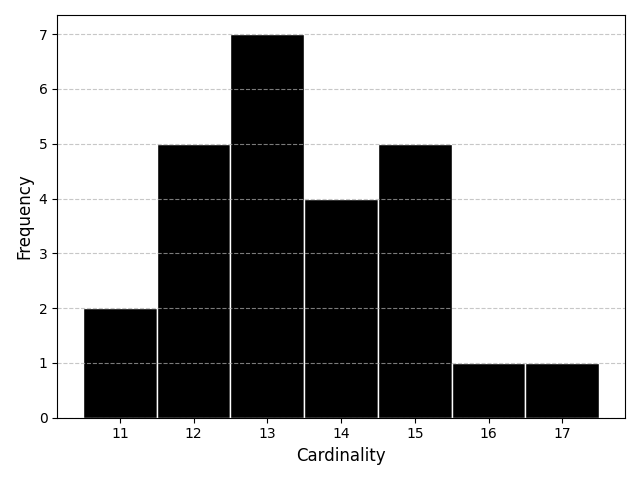
\includegraphics[width=\textwidth]{../figures/wine_cardinalities}
        \caption{Wine Dataset}
        \label{fig:wine_cardinalities}
    \end{subfigure}
    \hfill
    % Subfigure for Iris dataset
    \begin{subfigure}[b]{0.3\textwidth}
        \centering
        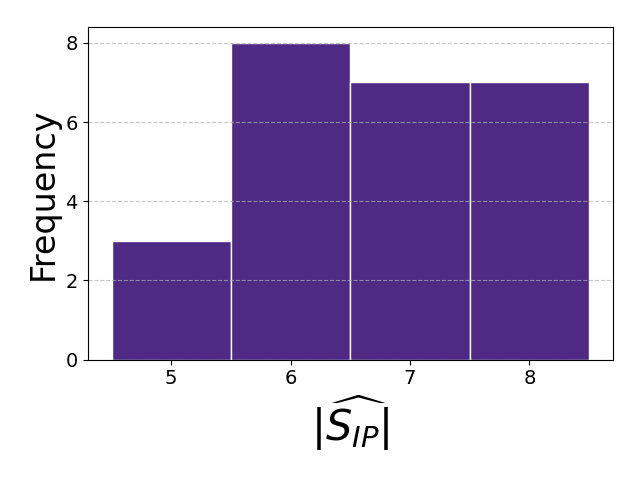
\includegraphics[width=\textwidth]{..//figures/iris_cardinalities}
        \caption{Iris Dataset}
        \label{fig:iris_cardinalities}
    \end{subfigure}
    \hfill
    % Subfigure for Ethanol dataset
    \begin{subfigure}[b]{0.3\textwidth}
        \centering
        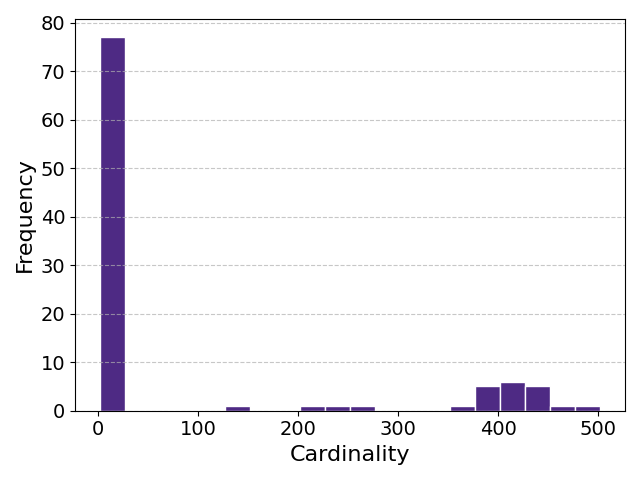
\includegraphics[width=\textwidth]{../figures/ethanol_cardinalities}
        \caption{Ethanol Dataset}
        \label{fig:ethanol_cardinalities}
    \end{subfigure}
    \caption{Support Cardinalities for Wine, Iris, and Ethanol datasets}
    \label{fig:support_cardinalities}
\end{figure}

\newpage

\subsection{Proposition \ref{prop:unitary_selection} deep dive}
\label{sec:deep_dive}

As mentioned in Section \ref{sec:discussion}, the conditions under which the restriction $P=D$ in Proposition \ref{prop:unitary_selection} may be relaxed are of theoretical and practical interest.
The results in Section \ref{sec:experiments} show that there are circumstances in which the \greedy~ performs better than \tsip, so clearly \tsip~ does not always achieve a global optimum.
Figure \ref{fig:comparison_losses} gives results on the line of inquiry about why this is the case based on the reasoning presented in Section \ref{sec:discussion}.
In these results a two-stage algorithm achieves the global optimum of a slightly different brute problem, namely brute optimization of the multitask basis pursuit penalty $\|\cdot \|_{1,2}$.
That is, brute search on $\|\cdot \|_{1,2}$ gives the same result as the two stage algorithm with brute search on $\|\cdot \|_{1,2}$ subsequent to isometry pursuit.
This suggests that failure to select the global optimum by \tsip~ is in fact only due to the mismatch between global optimums of brute optimization of the multitask penalty and the isometry loss given certain data.
Theoretical formalization, as well as investigation of what data configurations this equivalence holds for, is a logical follow-up.

\begin{figure}[t] % Place at the top of the page
    \centering
    % Top-left plot
    \begin{subfigure}[b]{0.45\textwidth}
        \centering
        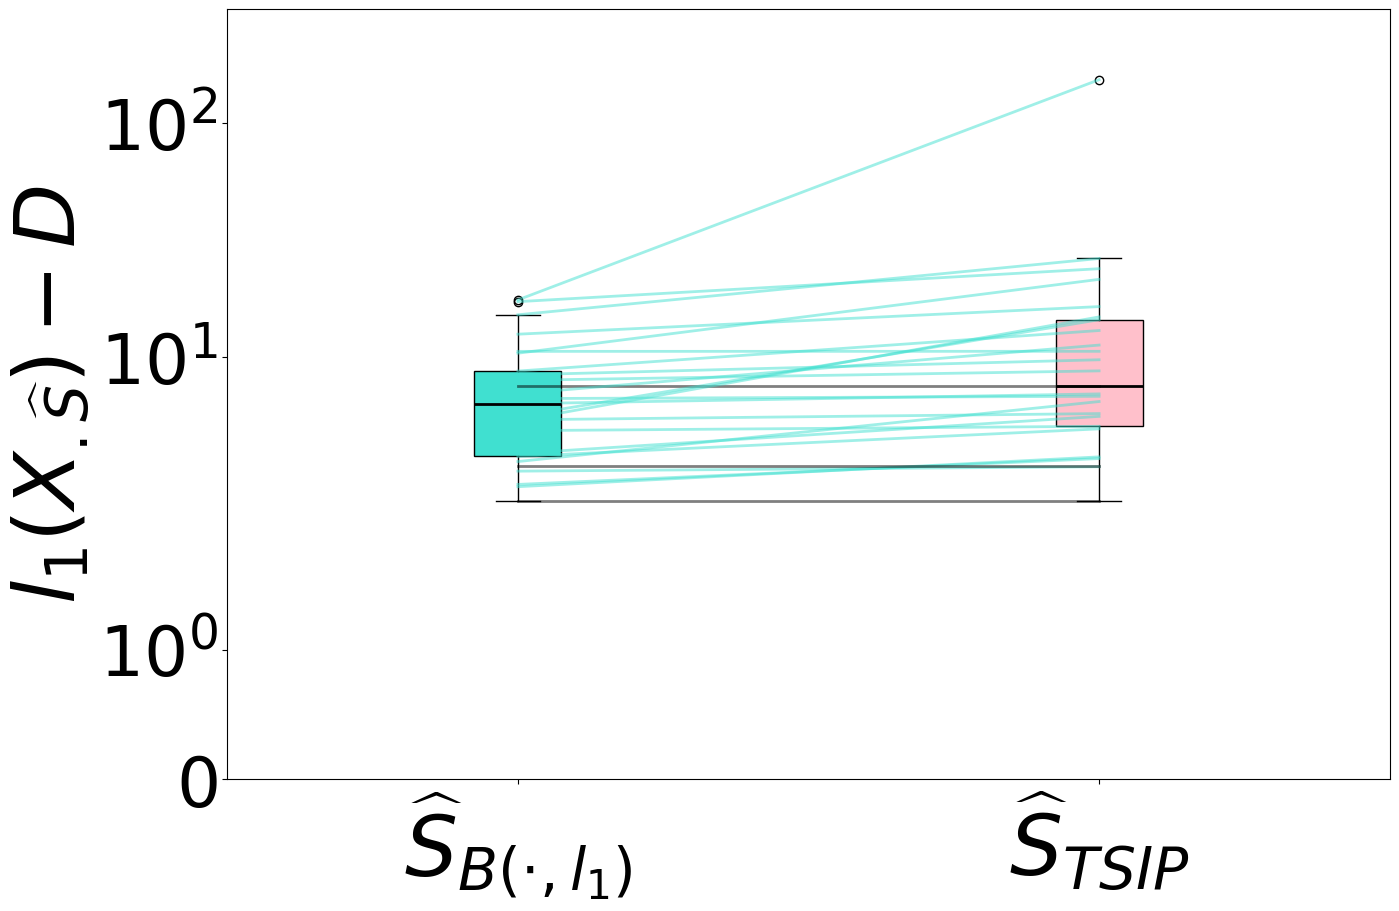
\includegraphics[width=\textwidth]{../figures/iris_standardized_0p1_1p0_isometry_losses}
        \caption{Iris Isometry Losses}
        \label{fig:iris_isometry_losses}
    \end{subfigure}
    \hfill
    % Top-right plot
    \begin{subfigure}[b]{0.45\textwidth}
        \centering
        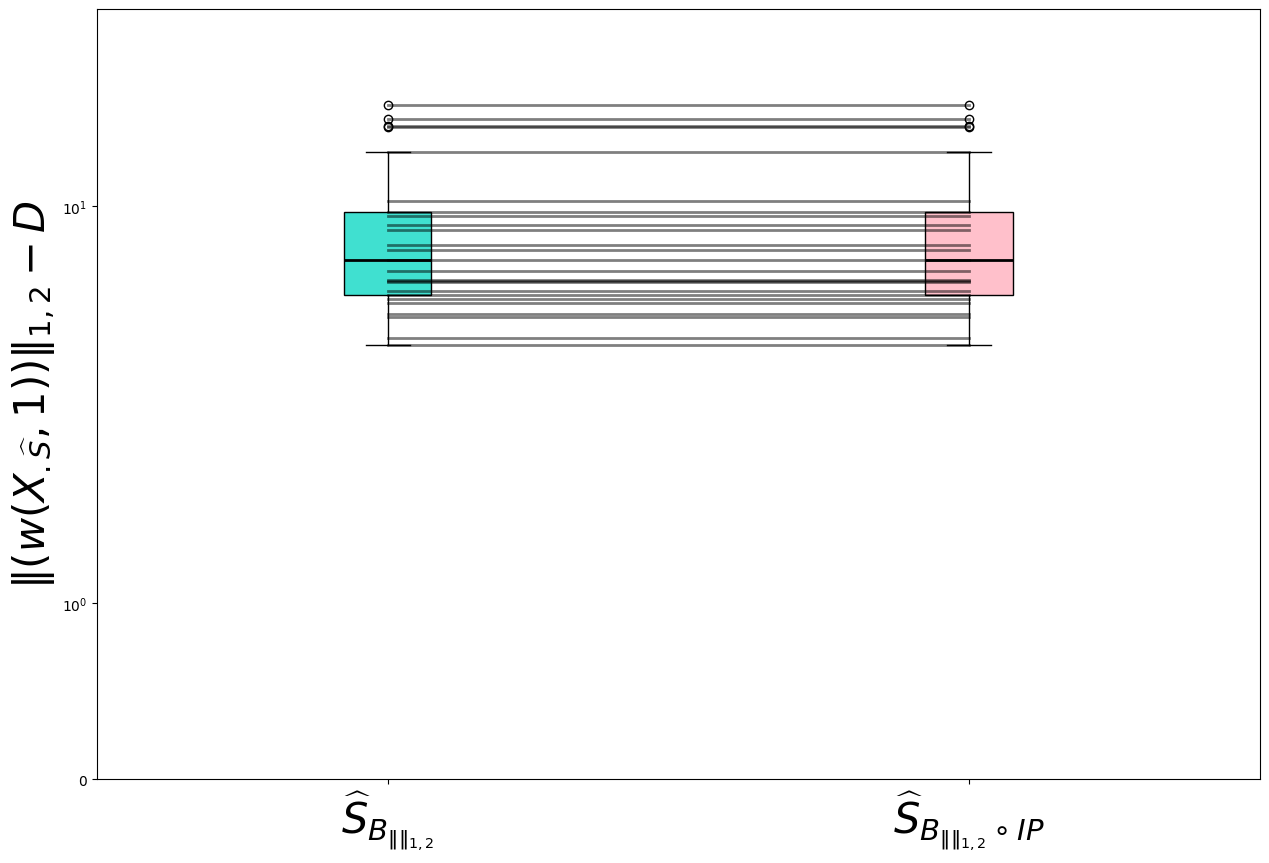
\includegraphics[width=\textwidth]{../figures/iris_standardized_0p1_1p0_group_lasso_losses}
        \caption{Iris Multitask Losses}
        \label{fig:iris_group_lasso_losses}
    \end{subfigure}

    \vspace{0.5cm} % Add vertical spacing between rows

    % Bottom-left plot
    \begin{subfigure}[b]{0.45\textwidth}
        \centering
        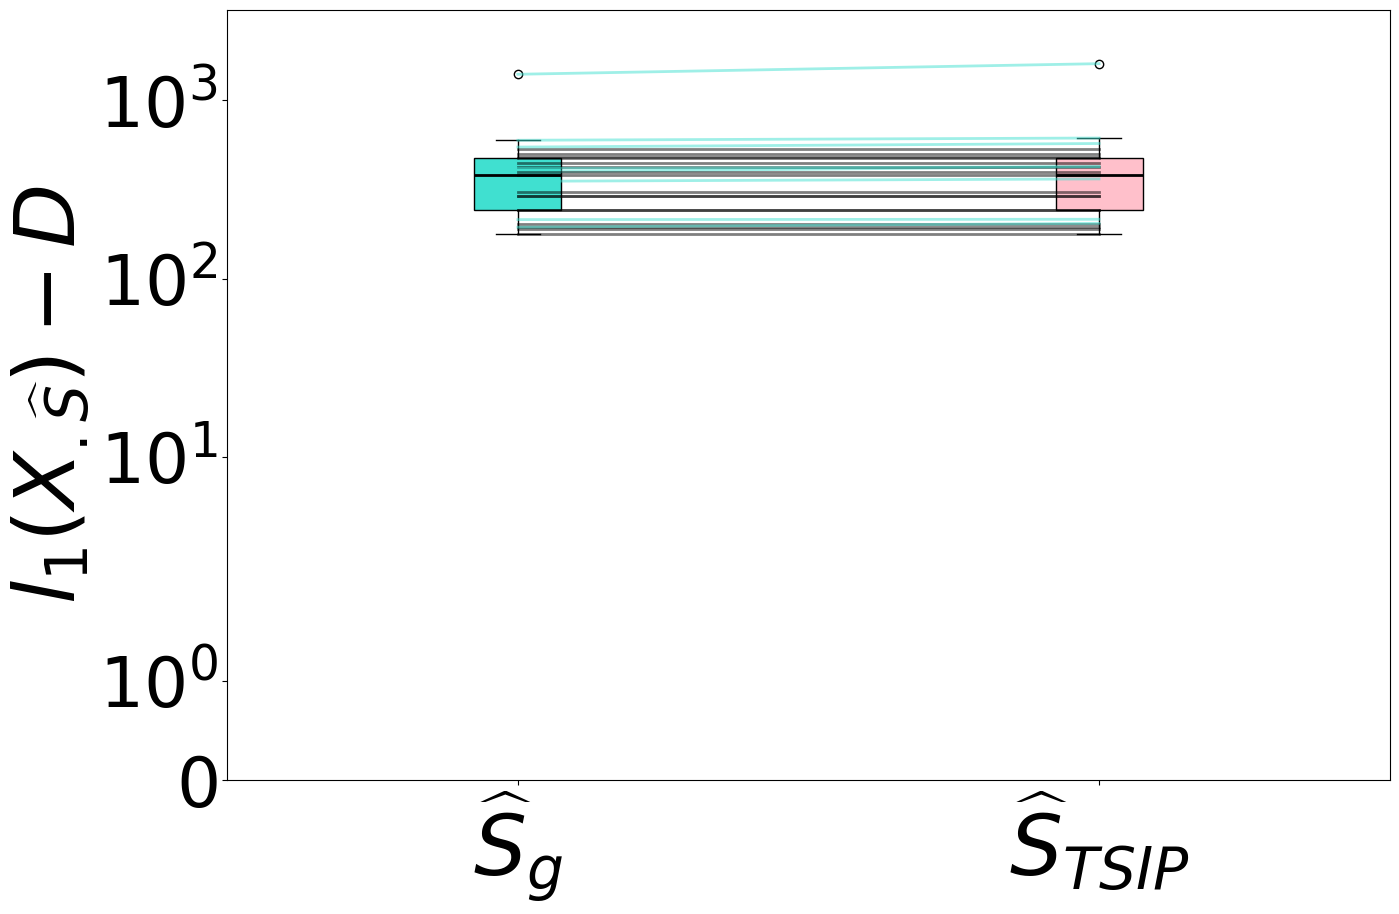
\includegraphics[width=\textwidth]{../figures/wine_standardized_0p1_1p0_isometry_losses}
        \caption{Wine Isometry Losses}
        \label{fig:wine_isometry_losses}
    \end{subfigure}
    \hfill
    % Bottom-right plot
    \begin{subfigure}[b]{0.45\textwidth}
        \centering
        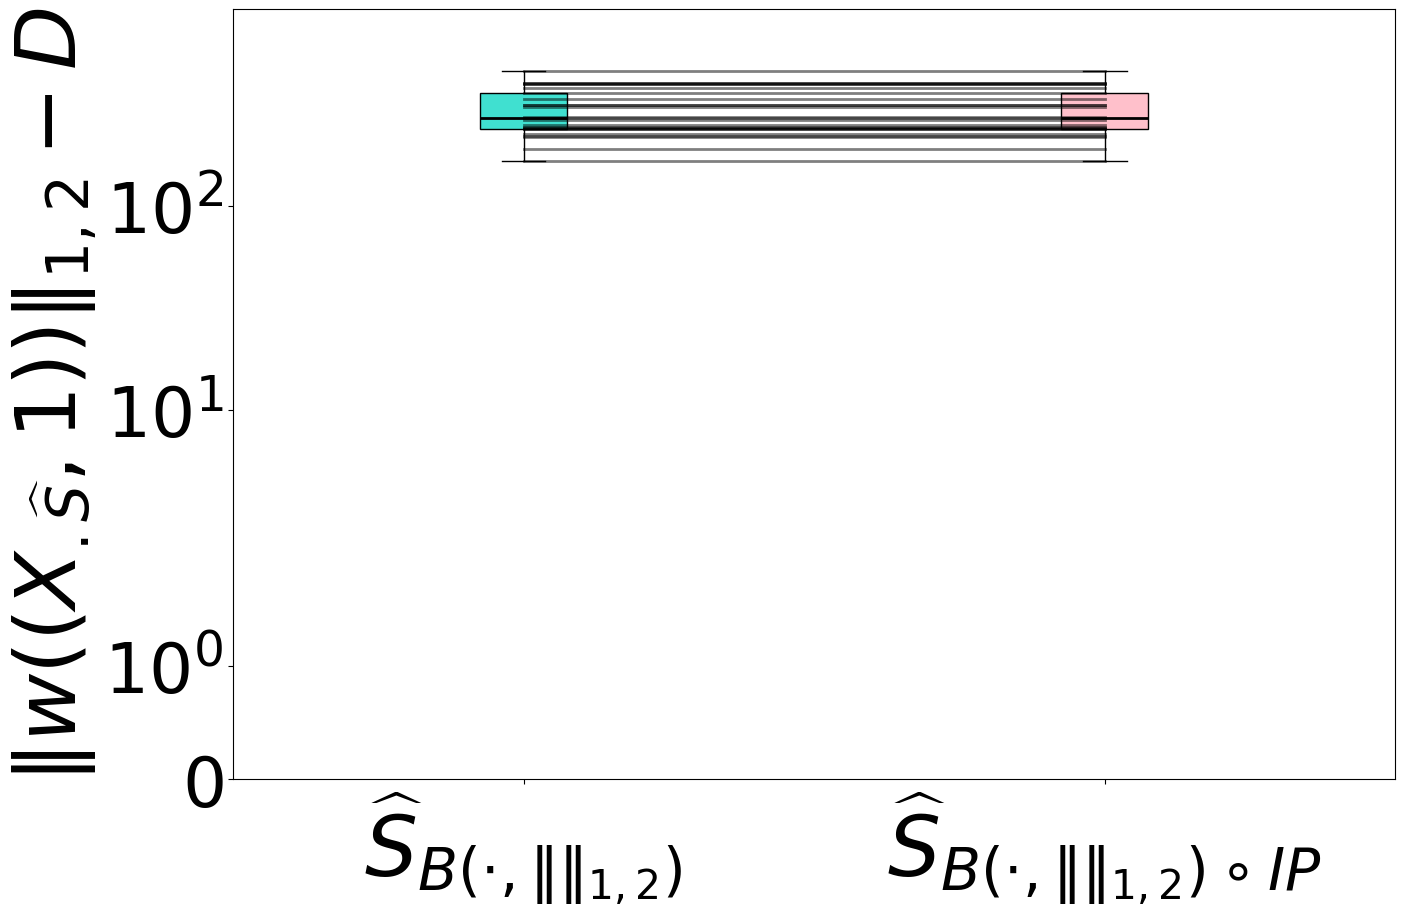
\includegraphics[width=\textwidth]{../figures/wine_standardized_0p1_1p0_group_lasso_losses}
        \caption{Wine Multitask Losses}
        \label{fig:wine_group_lasso_losses}
    \end{subfigure}
    \caption{Comparison of Isometry and Group Lasso Losses across $25$ replicates for randomly downsampled Iris and Wine Datasets with $(P,D) = (4,15)$ and $(13, 18)$, respectively.
    Note that this further downsampling compared with Section \ref{sec:experiments} was necessary to compute global minimizers of \brute.
    Lower brute losses are shown with turquoise, while lower two stage losses are shown with pink.
    Equal losses are shown with black lines.}
    \label{fig:comparison_losses}
\end{figure}

\newpage

\subsection{Timing}
\label{sec:timing}

While wall-time of algorithms is a non-theoretical quantity that depends on implementation details, it provides valuable context for practitioners.
We therefore report the following runtimes on a 2021 Macbook Pro.
The particularly high variance for brute force search in the second step of \tsip~ is likely due to the large cardinalities reported in Figure \ref{fig:support_cardinalities}.

\begin{table}[H]
\centering
\begin{tabular}{|c|c|c|c|}
\toprule
Name & IP & 2nd stage brute & Greedy \\
\midrule
Iris & 1.24 ± 0.02 & 0.00 ± 0.00 & 0.02 ± 0.00 \\
Wine & 2.32 ± 0.17 & 0.13 ± 0.12 & 0.03 ± 0.00 \\
Ethanol & 8.38 ± 0.57 & 0.55 ± 1.08 & 0.07 ± 0.01 \\
\bottomrule
\end{tabular}
\caption{Algorithm runtimes in seconds across replicates.}
\end{table}